\end{multicols*}

\mysection{The Obliterated}{forgotten-obliterated}

The nameless animals, elementals, and demons who populate \mylink{Limbo}{the-afterlife} can be summoned and commanded through your \mybold{Sovereignty}, a measure of your power to reach through the veil and bring forth their forms into \mylink{the Dream}{the-dream}. Their time with you is limited, existing only as long as you maintain \mylink{Concentration}{time-concentration}.

Other than their general type, the form the Obliterated take is only limited by your imagination - the more evocative, the better!  That said, there are a few basic parameters:


\callout {
    \mybullet {
        \item The Obliterated can only occupy a space roughly 3m in diameter. They could appear as a swarm of bees or a (small) herd of goats, but they would have to fit in a 3m circle.
        \item The Obliterated appear as spectral and indeterminate forms; they appears to always be shifting in appearance, and exude a ghostly and ethereal mist or smoke (they clearly do \mybold{not} look normal!).
        \item As stated above, the Obliterated exist for only as long as you maintain \mylink{Concentration}{time-concentration}. They are always summoned Close to you, and cannot move more than \mylink{Far-Away}{game-distance} from you. If your Concentration breaks, or they move more than Far-Away from you, they immediately Adjourn (see below).
        \item The Obliterated use your Sovereignty Die in Combat (see below). If the Obliterated ever reaches 0 Health, they immediately Adjourn.
        \item The Obliterated will obey you and only you (though some of the Damned may try to twist your words or intent).
        \item You can only summon Obliterated if you have their Fealty. You begin with the \mylink{Fealty of the Beasts}{forgotten-fealty-beasts}, but can earn the \mylink{Fealty of the Elements}{forgotten-fealty-elements} and \mylink{the Fealty of the Damned}{forgotten-fealty-damned} through \mylink{Advancement}{advancement-spriggan-virtues}.
    }
}


\mysubsection{Combat}{obliterated-combat}



Commanding an Obliterated to attack is considered a \mylink{Combat Action}{combat-combat-actions}. You make any Attack and Guard tries for the Obliterated under your control. When taking an Attack action, rather than rolling a Weapon Trait (\VIG, \DEX, etc.), you will instead roll one of the following die depending on your \MAX Sovereignty.

  \formula{Obliterated Attack/Guard Try}{
    \RO : Attack Die \PLUS Monster Weakness \PLUS your Level
  }
  

 \myctrtable{Y Y}{
    \thead{Sovereignty} & \thead{Attack Die} \\
  }{
      1 & d6 \\
      2-4 & d8 \\
      5-8 & d10 \\
      9 & d12
  }

  \myredbold{You can add the result of an \AWA try to the Obliterated's Attacking or Guarding try.}





The Health and damage die of the Obliterated depends on the amount of Sovereignty you use to create them (details are found in each Fealty below). 



\example{
    Oona, a first level Spriggan, is plundering an ancient aquatic temple with her Band. Creeping along the corridors, they hear guttural voices arguing around a dimly lit corner. They take a peek and see a handful of Deep Ones (Weakness: d24) fighting over a pile of rotting fish.

   As the rest of the Band prepares for combat, Oona decides to invoke the Fealty of Beasts to summon a swarm of bees, and commands them to attack. The Arbiter determines that the Deep Ones are Far-Away, and that the crew has \mylink{the Drop}{combat-drop} on them. Oona's Sovereignty is 2, so the swarm has 2 \HD, 6 Health (since they are weak), and will do d6 damage if they hit. The bees swarm around the Deep Ones; Oona must make a \RO try using a d8 (since her Sovereignty is 2) + d24 (Monster Weakness) + 1 (her level) for the swarm to hit their target(s). She must maintain \mylink{Concentration}{time-concentration} while the swarm attacks, or they will immediately Adjourn. She can summon one more Forgotten before she has to rest.
}

  \begin{multicols*}{2}

\mysubsection{Fealty of the Beasts}{forgotten-fealty-beasts}

\callout {
    Any Obliterated summoned through the Fealty of the Beasts has the \mylink{Trait: Zoological}{monster-trait-zoological} (this conveys no special effect).
}

Archaic and long extinct beasts inhabit the void of Limbo, and you know the ways to beckon them to you. The least powerful of these are Sprites, useful as spies and helpers.

\mybold{Sprites:}  A Sprite must take the shape of a single animal no bigger than a large dog; it can swim, crawl, or take flight as their shape dictates (an owl Sprite could fly but not swim). Sprites cannot deal damage directly, but they can interact with things if you wish them to. They can follow simple instructions ("get the key on the desk", "chew through these ropes", "spy on that man") but not more complex ones ("pick the lock").  The Sprite cannot speak, but you can share simple thoughts with them - you see what they see and hear what they hear, where appropriate. Sprites may be sent on missions a number of kilometers away, up to your \MAX Sovereignty. If the Sprite takes any damage, or if you stop Concentrating, it immediately Adjourns.

\mybold{Beasts:} A Beast is larger and more powerful. The type of beast is limited only by your imagination, though the Arbiter has the final OK, and it should be some kind of animal. The strength of the creature depends on your \MAX Sovereignty:

  \mytable{Y Y Y Y}{
    \thead{\footnotesize{Sov'rnty}} & \thead{\HD} & \thead{\footnotesize{Health}} & \thead{\footnotesize{Damage}} \\
  }{
      1 & 1 & Weak (3) & d4 \\
      2  & 2 & Weak (3) & d6 \\
      3+ & 3 & Weak (3) & d8 \\
  }

In addition, pick \mybold{one} of the following Traits for your Obliterated beast:


\mybold{Aquatic:} The Obliterated appears as a giant gar, mutant shark, octo-horse (like a seahorse combined with an octopus), etc. The Obliterated breathes water as air, and vice-versa i.e. if this Obliterated is removed from the water in any way, they begin \mylink{drowning}{movement-swimming}.

\mybold{Charging:} The Obliteraged appears as a small mammoth, spectral rhinoceros, two-headed bull, etc. It can spend an Action to charge somewhere Nearby. Every creature struck by the Obliterated in this way must Save vs. Doom or fall \mylink{Prone}{effect-prone}. It can run through a wooden wall but not a stone one (Arbiter's discretion). 

\mybold{Flying:} The Obliterated appears a megaowl, flock of seagulls, pterodactyl, etc. It can spend an Action moving one range step (Close to Nearby, Nearby to Far-away) up or down, and can hover in place.

\mybold{Leaping:} The Obliterated appears as a hefty bullfrog, trio of fraternal kangaroos, seven mammoth jumping spiders, etc. and can jump up to 10m forward, backward, or upward (equivalent of moving from Close to Nearby). If the Obliterated combines their jump with a \mylink{Bum Rush}{combat-deeds-bum-rush}, they deal +4 damage if they hit.

\mybold{Swarming:} The Obliterated appears as a swarm of bees, carpet of locusts, rat king, etc. and can attack all creatures Close to it in one Moment. It takes +4 damage per \DICE from attacks that affect \myital{all} Close creatures



\mysubsection{Fealty of the Elements}{forgotten-fealty-elements}

\callout{
    Any Obliterated summoned through the Fealty of the Elements has the \mylink{Trait: Elemental}{monster-trait-elemental}.
}

A constant stream of data pours into the unlit sphere of Limbo. In it swims the flotsam and jetsam of the elements, dissolving into nothingness, forgotten. You call to them across the void, and they manifest for you before flicking out of existence forever. Least of these are the Imps, useful as tools and distractions. 

\mybold{Imps:}  Imps appear somewhere Close or Nearby. The Imp is an elemental of a single type (fire, water, smoke, etc) and can take any form you wish, no bigger than a large dog. Imps cannot damage anything directly, though they can affect the environment appropriate to its type. For instance, you could summon a Fire Imp to run into a room to set something alight, or summon a Smoke Imp to stand in a doorway and hide something.  They can follow simple instructions ("jump into the hay (Fire)", "douse the fire (Water)", "blow out the torches (Air)") but not more complex ones ("burn the book the lich is carrying").  The Imp cannot speak, and unlike Sprites you cannot see what they see or hear what they hear (they make terrible spies). The Imp will respond to your (simple) mental commands if they are Close or Nearby to you; they cannot move further than Far-Away from you.  The Imp exists for as long as you Concentrate. If the Imp takes any damage or if you stop Concentrating, it immediately Adjourns.

\cbreak 

\mybold{Elementals:} Larger and more powerful elementals can be summoned as well. The type of Elemental is limited only by your imagination, though the Arbiter has the final OK, and it should take the form of an elemental power (a water wyrd, a salamander, etc). The strength of the creature depends on your \MAX Sovereignty: 


  \mytable{Y Y Y Y}{
    \thead{\footnotesize{Sov'rnty}} & \thead{\HD} & \thead{\footnotesize{Health}} & \thead{\footnotesize{Damage}} \\
  }{
      3 & 3 & Avg. (5) & d8 \\
      4  & 4 & Avg. (5) & d10 \\
      5+ & 5 & Avg. (5) & 2d6 \\
  }

Pick \mybold{any two} Traits from the \mylink{Fealty of Beasts}{forgotten-fealty-beasts} or the following:

\mybold{Amorphous:} The Obliterated appears as a gelatinous tetrahedron, swarm of radioactive static, humanoid shaped ball of mercury (\myital{Terminator 2}, \myital{The Abyss}, etc.). It can slip through cracks, go under doors, ooze up walls, hang on ceilings, etc. 

\mybold{Armored:} The Obliterated appears as a living boulder, elf of the Glacial Ice, magma encrusted pyramid, etc. It has an Armor of d8.

\mybold{Corrosive:} The Obliterated appears as a stream of acid, face in a (small) sandstorm, or vinegar drenched satyr. It removes 1 \UD of Armor whenever it successfully deals damage.

\mybold{Strong:} The Obliterated appears as a giant oak, brickwork cyclops, the Seven Dwarves, etc. It can perfom "feats of strength" (pick up wagons, smash through doors, lift gates and boulders, throw a cow over a wall ... OK. Throw a ship, pick up a house, punch through a castle wall ... not OK). It always wins \VIG contests (unless its opponent is also Strong).


\newpage

\mysubsection{Fealty of the Damned}{forgotten-fealty-damned}

\callout{
    Any Obliterated summoned through the Fealty of the Damned has the \mylink{Trait: Chaotic}{monster-trait-chaotic} and the \mylink{Trait: Otherworldly}{monster-trait-otherworldly}
}

You have gazed long into the abyss of Limbo; your vision has descended into it, mapped it, and found the paths to the Other Side. It is filled with chaos, destruction, and death, and ruled by creatures born of the Void. Lashing them with ethereal chains, you pull them back across the singularity to serve you, before casting them back to Hell. The weakest of these are the Gremlins, creatures of pure chaos and destruction, whose appetites are severely curtailed by their small size.

\mybold{Gremlins:} A few dozen Gremlins appear at a point Close or Nearby. Gremlins cannot damage anything directly, and only exist to cause havoc and chaos. You can partially guide them, but they are generally under the control of the Arbiter. When they are summoned they immediately run in different directions (but won't move further than Far-Away from you) and cause as many problems as they possibly can - unbuckle belts, set things on fire, cut ropes, smash pottery, scream and kick in the middle of the floor, etc.  They may or may not follow instructions (Arbiter's discretion.  If you're stuck, roll a die and have them react randomly). Gremlins can speak and imitate voices if they desire. You can see what they see and hear what they hear, but it's generally unpleasant to do so. The Gremlins exists for as long as you Concentrate. If the Gremlins takes any damage or if you stop Concentrating, they immediately Adjourn.


\mybold{The Damned:} Larger and more powerful Demons and Devils can be summoned as well. The type of Damned is limited only by your imagination, though the Arbiter has the final OK, and it should take the form of a demon of some sort (a vrock, nightgaunt, etc). The strength of the creature depends on your \MAX Sovereignty:

    \mytable{Y Y Y Y}{
    \thead{\footnotesize{Sov'rnty}} & \thead{\HD} & \thead{\footnotesize{Health}} & \thead{\footnotesize{Damage}} \\
  }{
      5 & 5 & Str. (7) & 2d6 \\
      6  & 6 & Str. (7) & d6+d8 \\
      7+ & 7 & Str. (7) & 2d8 \\
  }

Pick \mybold{any three} Traits from the Fealty of the  Beasts, Fealty of the Elements, or the following:

\mybold{Alien:} The Obliterated appears as a Shoggoth, Yuggothian Fungi, Vinz Clortho, etc. Its appearance causes an immediate \mylink{Insanity}{adventurer-kismet-insanity} try and / or Morale check for all Allies and Monsters Close to the point of the summoning. It is immune to \mylink{Toxins}{malignants-toxins} and \mylink{Diseases}{vulgate-medicine-diseases}.

\mybold{Berserk:} The Obliterated appears as an eight-armed carnivorous white ape, two-headed Vrock, swarm of land pirhana, etc. It will fight until the Bottom of the next Moment \myital{after} it is reduced to 0 Health.

\mybold{Draconic:} The Obliterated appears as a red drake, drowned sultan, puff-cheeked bullfrog, etc. It can breathe out a breath of any element you choose (appropriate to its type) once per Combat. This breath affects all Close OR Nearby (Distinct) Allies and Monsters, and hits automatically. The breath deals your \MAX Sovereignty x2 damage (Save for half).

\mybold{Tactical:} The Obliterated appears as a black-armored knight, red Devil, Ba'al raiding party, etc. It deals +3 damage if it remains Close to you, and an additional +1 damage for each Close Ally (to itself). For example, if you and 3 Allies were Close to this Obliterated, it would deal +6 damage.

\begin{center}
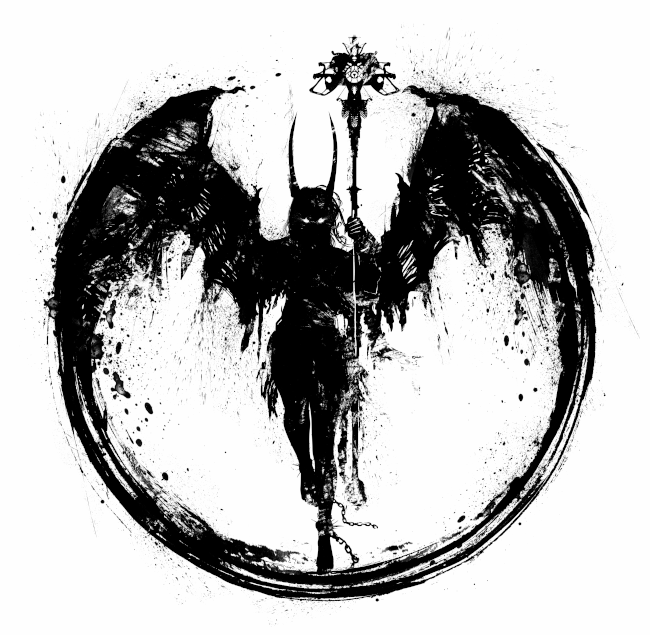
\includegraphics[scale=.35]{remembrance/TheDamned}
\end{center}

